\documentclass{article}
\usepackage[margin=1in]{geometry}
\usepackage{amsmath,amsfonts}
\usepackage{listings}
\usepackage{color}
\usepackage{verbatim}
\usepackage{graphicx}
\usepackage{float}
\usepackage{pdfpages}\usepackage[section]{placeins}
\usepackage{tikz}
\usetikzlibrary{backgrounds}

\definecolor{dkgreen}{rgb}{0,0.6,0}
\definecolor{gray}{rgb}{0.5,0.5,0.5}
\definecolor{mauve}{rgb}{0.58,0,0.82}
\definecolor{black}{rgb}{0,0,0}

\title{\textsc{\textbf{Business and Outreach Plan}}}
\author{\textsc{FTC Team 4278 {\color{dkgreen}de.evolution}}}
\date{}

\makeatletter

\tikzset{%
  fancy quotes/.style={
    text width=\fq@width pt,
    align=justify,
    inner sep=1em,
    anchor=north west,
    minimum width=\textwidth,
  },
  fancy quotes width/.initial={.8\textwidth},
  fancy quotes marks/.style={
    scale=6,
    text=black,
    inner sep=0pt,
  },
  fancy quotes opening/.style={
    fancy quotes marks,
  },
  fancy quotes closing/.style={
    fancy quotes marks,
  },
  fancy quotes background/.style={
    show background rectangle,
    inner frame xsep=0pt,
    background rectangle/.style={
      fill=gray!25,
      rounded corners,
    },
  }
}

\newenvironment{fancyquotes}[1][]{%
\noindent
\tikzpicture[fancy quotes background]
\node[fancy quotes opening,anchor=north west] (fq@ul) at (0,0) {``};
\tikz@scan@one@point\pgfutil@firstofone(fq@ul.east)
\pgfmathsetmacro{\fq@width}{\textwidth - 2*\pgf@x}
\node[fancy quotes,#1] (fq@txt) at (fq@ul.north west) \bgroup}
{\egroup;
\node[overlay,fancy quotes closing,anchor=east] at (fq@txt.south east) {''};
\endtikzpicture}

\makeatother

\begin{document}
\maketitle

\newpage\tableofcontents\newpage\setlength{\parskip}{4pt}

	\section{Business Plan}

\subsection{Team Mission}

Our mission is to create a community of student and adult leaders passionate about science, technology and engineering. We aim to provide an environment centered around fostering intellectual creativity, cooperation, and competition, as we all work together to develop critical thinking, problem solving, and team building skills. In addition, our goal is to make a positive impact in our school and general communities, while promoting the ideals of FIRST. 

\subsection{Team Origin}

Our team was founded in September of 2010 at Canyon Crest Academy in San Diego, California as part of the CCA Robotics Program and meets afterschool in a team member’s garage. De.Evolution Team 4278 has maintained between 7-10 members over the last four years but actually functions as part of a greater business model including three FTC teams and One FRC team. Thanks to combined resources and team coordination our influence in the community has skyrocketed, allowing us to acquire more resources, better workspaces for our class and FRC teams as well as awesome mentors. In addition, alumni team members have come back to share their knowledge and experience with both FRC and FTC teams. 

One of the challenges our program has had to overcome over the years is a lack of facilities and resources. Throughout the lifetime of our team, we’ve had to make do with small spaces and a lack of access to more advanced tools. Thanks to a robust model for sponsorship and fundraising we have seen significant growth in our design process this year, in which the vision for our robot was completed quickly and efficiently using 3D modeling/design and advanced materials. While we began with a limited set of skills and experiences, through our failures we have been able to come up with better designs in a much shorter amount of time. We’ve successfully developed a program that promotes the values of FIRST to students and our community, and will continue to for years to come.

\subsection{Organizational Structure}

[Insert orgchart]

\subsection{Relationships}

As part of the Canyon Crest Academy Robotics Program our team takes the relationships between our students, mentors, and community very seriously, and we aim to be continuously improving our connections with them. Team 4278 leaders work within the organizational structure above to expand access to STEM within our entire school and the community. As part of this business model we plan to offer nights during the year in conjunction with our other teams where students and parents can come on campus to our student-run cafe to enjoy food and beverages while seeing demonstrations of robots and learning more about the different robotics programs at our school. Furthermore, we plan to sell special fan shirts to enable fellow students and teachers to show their support for the teams, serving the teams financially as well as fostering school spirit. 

We often partner with the Humanities Conservatory at our school for assistance with writing grants and seeking out sponsors. Corporate support is allocated to each of the four teams within the program. We are grateful for the continued support of our veteran sponsors, and are actively looking for new contacts through our local community. This year, we’ve reached out to four additional companies and are continually seeking more in pursuit of this goal. We also join with other facets of our school during the annual pep rally and Quest/STEM Nights to get people excited about STEM. In the spirit of Coopertition, we often partner with various FTC and FRC teams in our area; as we exchange knowledge, resources and experiences, we gain valuable input and perspectives that benefit everyone. 

We are constantly on the lookout to plan awesome team building events and trips that give us the chance to grow closer as a group. Overall, we really value the relationships within our team and in our community, and we hope to strengthen these over time. 

\subsection{Deployment of Resources}

Our team greatly values our community and aims to engage it in activities that further the appreciation of science, technology, engineering, and mathematics. Because of this, we have specifically organized our resources to maximize our ability to both inform and involve our community in STEM subjects. We regularly excite members in our school through events like Club Day, Quest Night and Parent Night, where we show our robot to a large amount of people and get them interested in robotics. Furthermore, we plan and participate in school-wide events like our school’s biannual pep rally to stimulate fascination amongst the student body. 

We also aim to spread the word of FIRST to middle and elementary schools with a goal of exposing students to STEM. Our objective in demonstrating at schools is to both start new FLL and FTC teams and get kids interested in robotics, as well as partner with already existing FTC and FLL teams as mentors. By mentoring others, we challenge team members to expand their skillsets and solidify the knowledge they’ve already acquired. As a team, our goal is to spread the message of FIRST everywhere we can and to create communities for students, parents, and teachers aiming to improve their critical thinking, team building, and problem solving skills, and support science, technology, engineering and mathematics.

\subsection{Future Plans}

While planning our next three years, our team’s main goals are to promote the core values of FIRST, to encourage the growth of a supporting and excited community, and to make an impact outside of robotics and engineering related areas. For instance, in order to establish connections between people through robotics, we plan to host fundraisers at various restaurants on the first Tuesday of every month. By doing this, we aim to not only raise funds to continue the impact of our team, but also bring together a community focused on STEM by being a reliable location for friends and family to meet each other while actively supporting the team. We also plan to continue to grow our relationship with the art programs at our school, to involve them in actively supporting our team and FIRST. 

We plan to partner with our cinema and art conservatories to help our marketing team expand its capabilities in the realms of graphics and videography. Outside of competition and robotics, our team values making an impact within the community. We plan to partner with other teams in our area to organize regular beach cleanups along the coast in order to help the environment. Furthermore, we plan to continue to reach out to companies for grants to allow us to grow our team and reach even more students in more diverse ways. Our team is focused on engaging our community both inside and outside of school, all in the name of STEM, and over the next three years we believe we can build relationships more effectively with the people around us.

\subsection{Financial Statement}

Income:

\begin{tabular}{|c|c|}
\hline
Starting Balance & \texttt{\$3,795.78} \\
\hline
\end{tabular}   \newpage
\section{Outreach}
As a team, de.evolution believes that robotics is more than just the engineering. Our first year as a team we saw that the other FTC team at our school, Domo Arigato, was entirely seniors and we were sad that it was going to disappear. This inspired us to try and spread robotics to the younger students and have people involved to keep robotics teams going and to propogate the message of FIRST throughout our community. We have started a robotics class at our high school which has turned into the team Domo Arigato. Due to the popularity of the class a second class, and subsequently an FTC team, has been started. Both the Robo Ravens and Domo Arigato, along with our own team, de.evolution, work hard to start a robotics and engineering culture at our school. The section will be structured as follows, we will begin by listing our community outreach and will in the subsequent subsections go into further detail about some of the more important work we do

\subsection{Community Outreach}
As a team, de.evolution has tried to do a lot to help spread the ideas of FIRST, robotics and engineering. The following is an extensive list of some of the community outreach that we have done:

\begin{enumerate}
\item Robotics demos to elementary school students at Solana Pacific Elementary, Del Mar Heights Elementary, Rancho Santa Fe Elementary
\item PTC World demo in June 2013
\item Mentoring of the three Islamic School of San Diego FLL teams 
\item Sister team of the San Dieguito Academy FTC teams Paradox Squared and Paradox Cubed
\item Demo for school board \& superintendent – sponsored building/engineering production district-wide with bond measure
\item Hosted Robotics Week at CCA in coordination with Domo Arigato
\item Publication in newspapers \& press releases about stem/robotics
\item Publication in school's magazines
\item Over 20\% of school has become involved with the FIRST robotics programs after the inception of our team
\item Inspired the FIRST robotics classes
\item Incorporating art and conservatory at CCA with the robotics program
\item Incorporating the humanities conservatory at CCA with the robotics teams
\item Working with TEDxYouth@SanDiego to spread robotics to the students in San Diego
\item Hosted small scrimmages at home
\item Hosting fundraisers at Souplantation for FIRST robotics
\item Attended and presented at Rotary meetings to show our community the influence of robotics
\end{enumerate}

\subsection{Helping other teams online}
As the majority of the members on our team are also on the FRC team \underline{The Aluminum Narwhals} we realize that having online support is one of the best ways to debug and learn about robotics. Chief Delphi, one of the prominent places for online FIRST discussion, is very popular among FRC teams. However, FTC teams do not have nearly as much online support as they may need or like. As a team we have shifted a lot of our focus to helping teams online. We have open-sourced all of our code and have created code tutorials to help out many other teams. In specific we have helped teams in the following ways:

\subsubsection{Syntax Error code optimization assistance}

At a San Diego regional qualification competition, we entered a discussion with team 6077, Syntax Error, about code optimization. We were sharing our varied tricks which were used in code, and through discussion, it became clear that there were a couple points they were particularly interested in implementing. We passed them some contact information, and later received an email from them:

\begin{lstlisting}
Hey Noah,

We're interested in optimizing the speed of our teleop code, and I know you had mentioned at the tournament that you guys XOR-ed the joystick values to determine when the values had changed--allowing you to skip checks when things weren't changing. Could you please go into more depth as to how you achieved this? Did you directly modify joystickdriver.c? Which values should we be XOR-ing exactly?

Thanks,
-Collin 
\end{lstlisting}

We wrote out a document generally detailing the approaches we took when optimizing our teleoperated code. My response was the following PDF file:

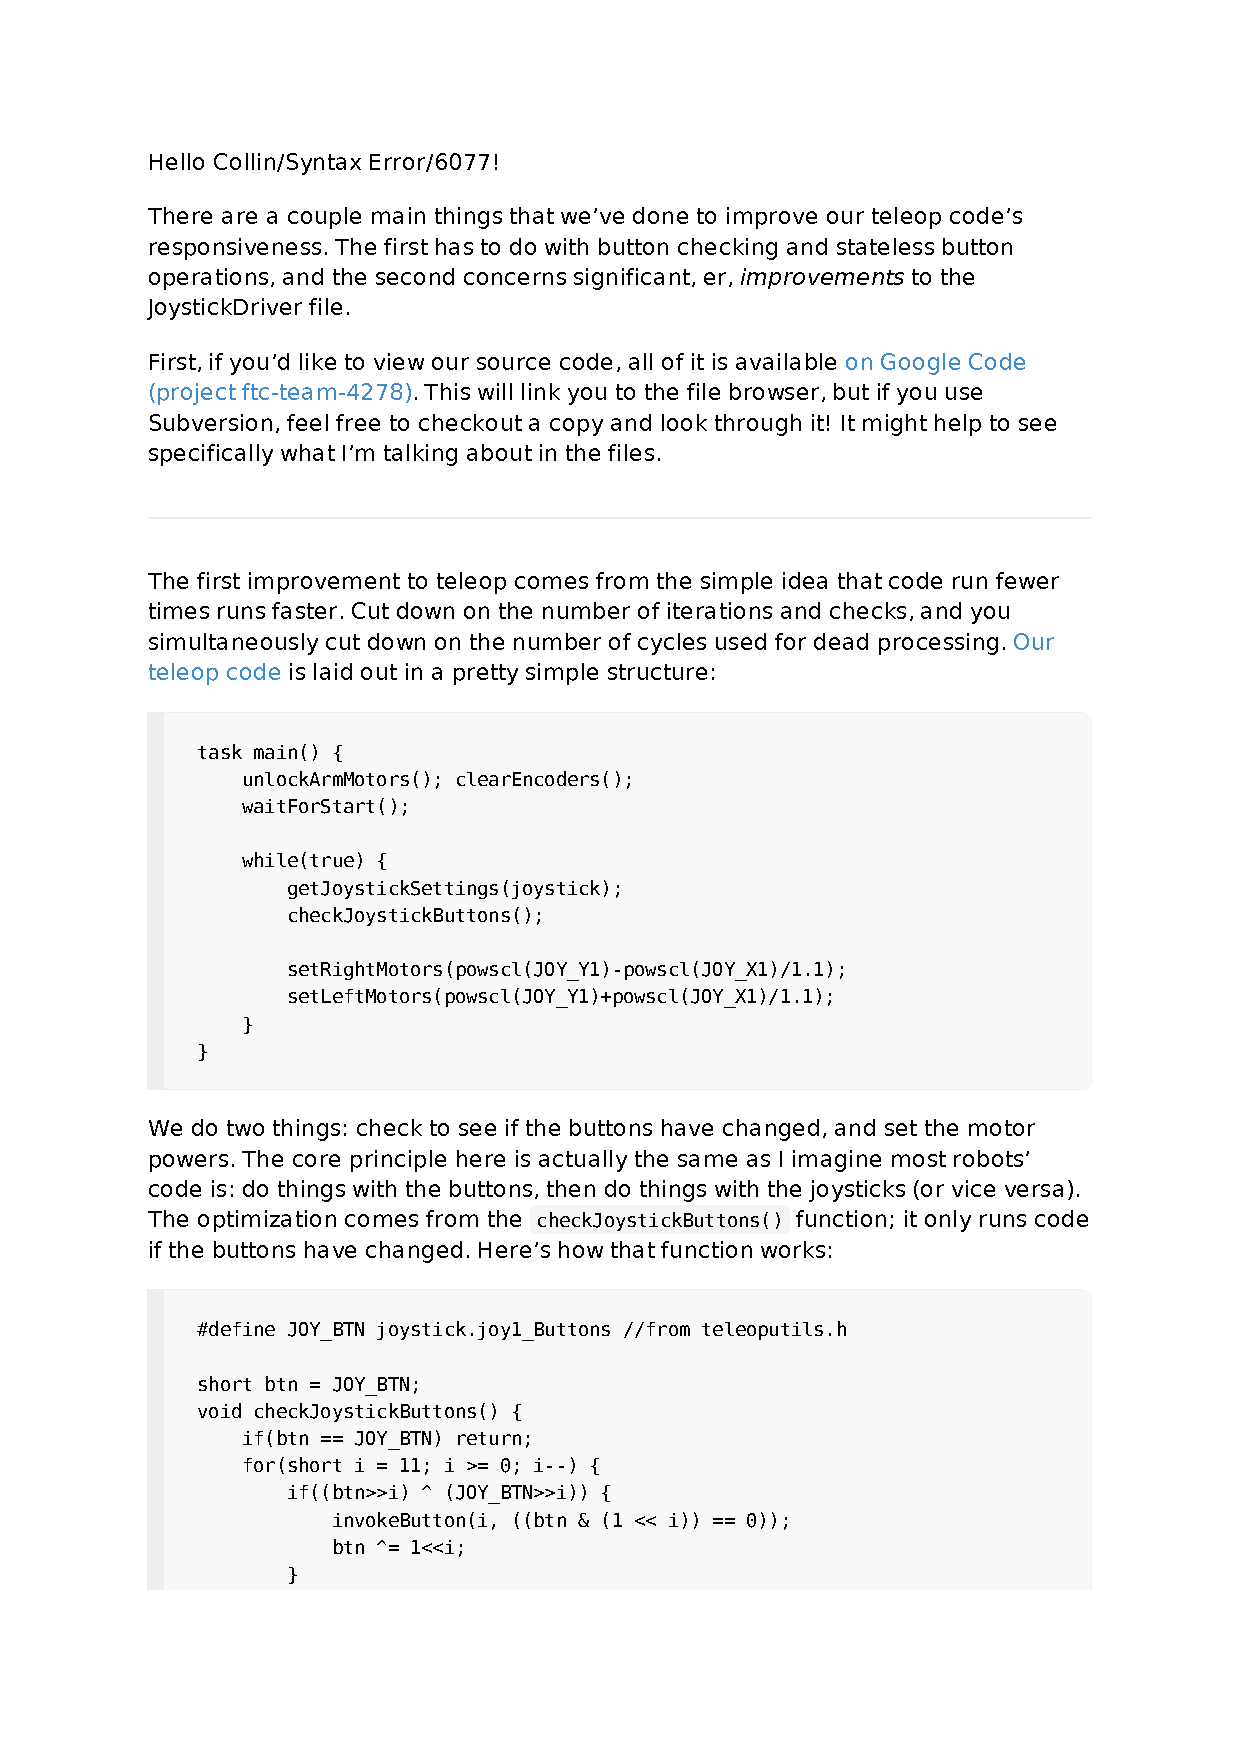
\includepdf[pages={1-2}]{SyntaxError.pdf}

The aim was to create an easy-to-follow guide for someone with experience to optimize the teleoperated program. To our enjoyment, they reported significant increases in response time on their controller.

\subsubsection{Reddit}

\subsection{Mentoring of FLL teams}
Our team aided the Islamic School of San Diego's FLL Teams during their rookie years by mentoring the young kids on robotics and the engineering design process in general. Our students voluntarily watched over the excited and energetic children, assisted in teaching them key concepts, and created useful PowerPoint presentations that were presented to further educate the FLL teams.

In each meeting, the FLL teams was taught a concept and then given time to build something from LEGOs using their newfound knowledge. Since our de.evolution volunteers were there, the FLL leader could split the team into small groups with a mentor or leader helping each group. Another advantage of having an FTC mentor available was that the volunteer could lead the team while the leader temporarily prepared the next lesson or dealt with other essential tasks. It relieved the leader of FLL and kept everything running smoothly.

The lessons taught the eager and energetic students about what causes earthquakes and the destruction that they inflict. This understanding supported the kids in cooperatively creating ideas for a machine to aid anyone who recently experienced a devastating disaster. The mentors also educated the group about the engineering design process to assist them in efficiently building a better solution when they were ready to begin fabrication of their product.

We found that mentoring FLL teams has not only allowed us to teach the students a lot about robotics, but we gained valuable experiences by doing so.
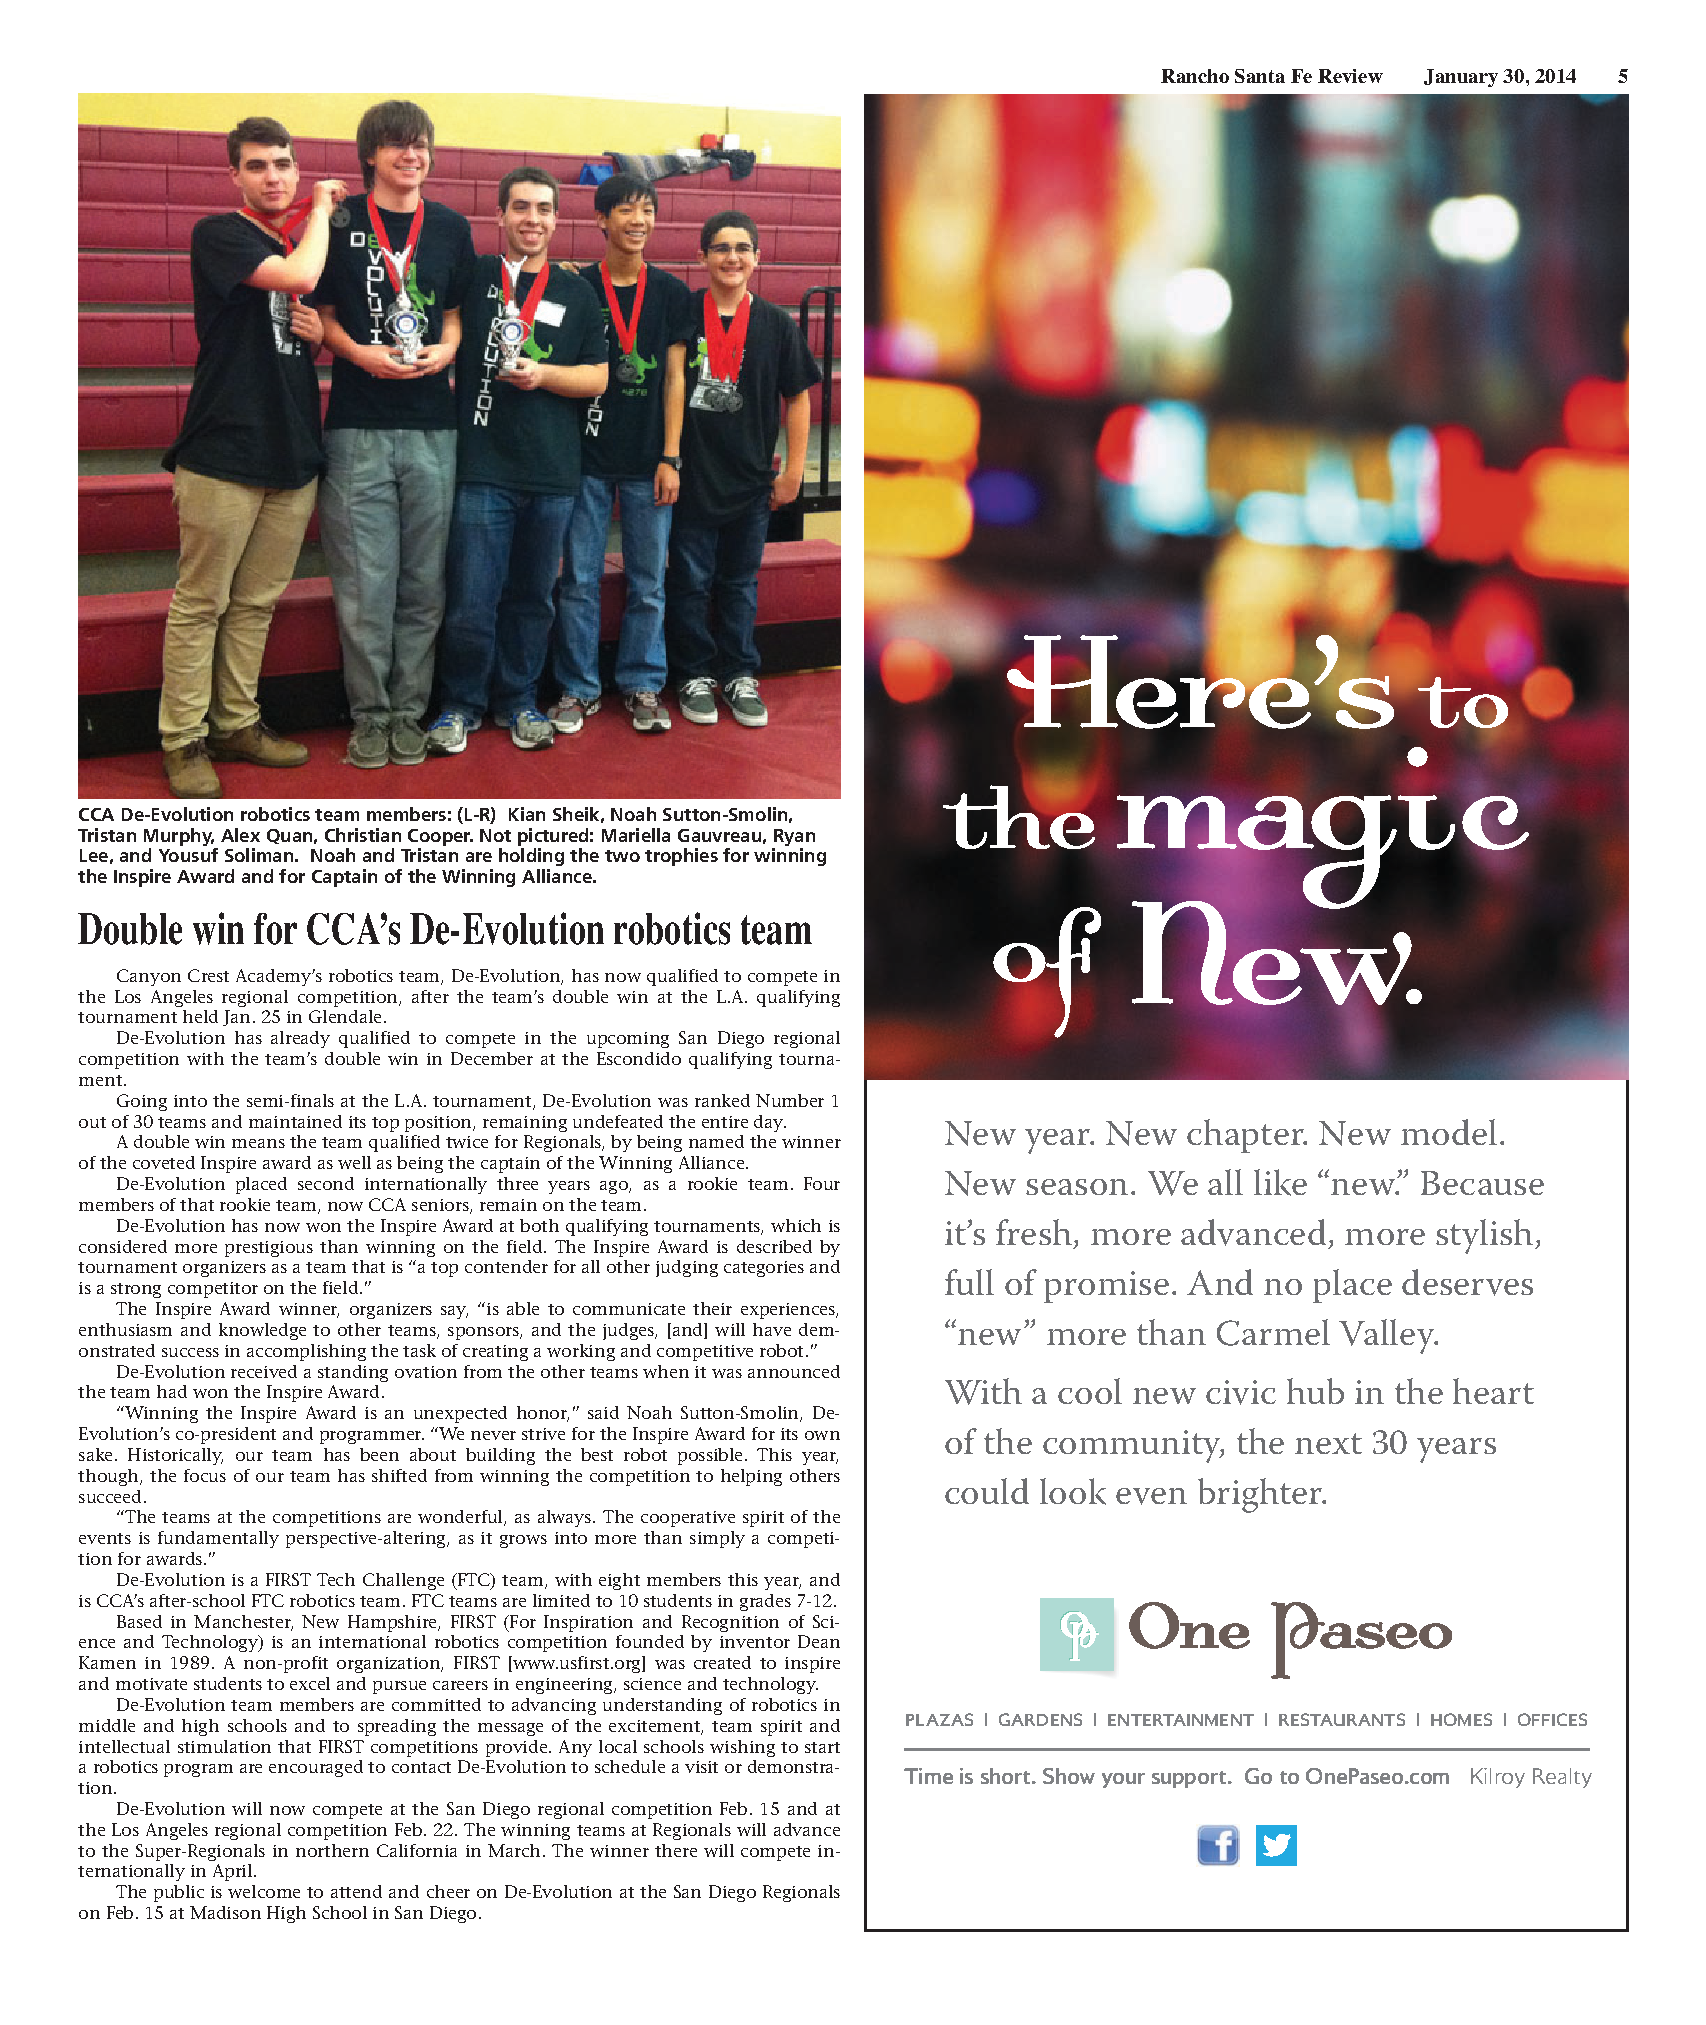
\includepdf[pages={-}]{DoubleWinNewspaper.pdf}

   \newpage
\end{document}